\documentclass{article}
\usepackage[utf8]{inputenc}
\usepackage{tikz}
\usetikzlibrary{positioning}

\title{IML Exam}
\author{David Ponarovsky}
\date{July 2021}
\usepackage{braket}
\usepackage[a4paper, total={6in, 8in}]{geometry}
\usepackage{amsmath}
\usepackage{amsfonts}
\begin{document}

\newcommand{\xy}{\mathbf{x^{\prime}}, \mathbf{y^{\prime}}}
\newcommand{\xxo }{ \mathbf{x^{\prime}}_1 }
\newcommand{\zoo}{ \begin{bmatrix} 
\frac{1}{2}\cdot(-1)^{z_1} + \frac{1}{3}\cdot(-1) ^{z_3} \\
\frac{1}{2}\cdot(-1)^{z_2} + \frac{1}{3}\cdot(-1) ^{z_4} 
\end{bmatrix}  }
\maketitle

\section{IML Exam}
\paragraph{Q1 ANN VC dim}
The following net contains \( n \) neurons in the input layer and a pair of neurons in the middle layer. One of the neurons in the middle layer is connected to all of the input neurons, while the other is connected only to the first input neuron.  Let the activation function be \( \sigma_{i} (x) = sign(x + b_{i}) \) what is the \( VC \dim \) of the network? 

\paragraph{}

\tikzset{%
  every neuron/.style={
    circle,
    draw,
    minimum size=0.8cm
  },
  neuron missing/.style={
    draw=none, 
    scale=2,
    text height=0.25cm,
    execute at begin node=\color{black}$\vdots$
  },
}

\begin{tikzpicture}[x=1.5cm, y=1cm, >=stealth]

\foreach \m/\l [count=\y] in {1,2,3,4,missing,5}
  \node [every neuron/.try, neuron \m/.try] (input-\m) at (1 ,1-\y) {};

% \node [every neuron/.try, neuron 6.try] (middle-1) at (3 ,-1) {};
\node [every neuron/.try, neuron 7.try] (middle-2) at (3 ,-3) {};
\node [every neuron/.try, neuron 7.try] (out-1) at (5 ,-2) {};

\foreach \l [count=\i] in {1,2,3,4, 5}
  \draw [<-] (input-\i) -- ++(-1,0)
    node [above, midway] {$I_\i$};
    
\draw [->] (out-1) -- ++(1,0)
    node [above, midway] {$O$};

\foreach \y [count=\yi] in {1,2,3,4,5}  
%   \foreach \j in {1,...,2}
       \pgfmathtruncatemacro{\cur}{\y}
       \pgfmathtruncatemacro{\next}{\y + 1}
      \draw [->](input-\cur) -- (middle-2);
    %   \draw [->] (input-\cur) to [out=50,in=160] (input-5);    


% \foreach \y [count=\yi] in {1,2,3}  
% %   \foreach \j in {1,...,2}
%       \pgfmathtruncatemacro{\cur}{\y}
%       \pgfmathtruncatemacro{\next}{\y + 1}
%     %   \draw [->](input-\cur) -- (input-\next)
%       \draw [->] (input-1) to [out=50,in=130] (input-\next);    
% \draw [->](input-1) -- (input-5);
\draw [->] (input-1) to (out-1);
% \draw [->] (middle-1) to (out-1);
\draw [->] (middle-2) to (out-1);
    % \draw [->] (input-\y) -- (input-(1+\y));



\foreach \l [count=\x from 0] in {Input, Ouput}
  \node [align=center, above] at (1 + \x*4,0.5) {\l \\ layer};

\end{tikzpicture}
\paragraph{Q1 Solution}

the form of hypothesis class is \[ h( \mathbf{x} ) = sign\left( w^{(2)}_{1}x_1 +w^{(2)}_{2} sign\left(   \braket{ \mathbf{w^{(1)}},\mathbf{x} } + b_1 \right) + b_2 \right)  \] where \( \mathbf{w^{(1)} } \) and \( b_1 \) are the parameters of the middle layer and the \( w^{(2} \) is the weight of the synapses which connect the first neuron and the middle neuron to the output neuron. \( b_2 \) is the parameter of output layer activation function. Clearly the middle layer is just an hyper plane, therefore it shatters a set of \( n + 1 \) points, denote that set by \( S \). 
let choose \( w^{(2)}_2= \frac{1}{2} \), \(|b_2| \le \frac{1}{4} \) and \( w^{(2)}_1 \) such that \( |w^{(2)}_1| \le \frac{1}{4\cdot \max_{x \in S} {|x_1|}} \), on the one hand for every \( x \in  S\) we get that \( h(x) = sign\left(   \braket{\mathbf{w^{(1)}},\mathbf{x} } + b_1 \right) \), on the other, we could choose points \( \mathbf{x^{\prime}}, \mathbf{y^{\prime}}\), such that \( |\mathbf{x^{\prime}}_1| = 4 \cdot \max_{x \in S} {|x_1|} \) and \( \mathbf{y^{\prime}}_1 = 100\frac{b}{w^{(2)}_1}- \mathbf{x^{\prime}}_1\). let's denote by \( z_1 , z_1 \in \{0,1\} \) the output of the middle layer over \( \xy \) and by \( z_3, z_4 \in \{0,1\} \) the excepted classification of \( h\), than we could reduce the problem to find a solution for the given equation system:
\[
\begin{bmatrix}
\xxo & 1 \\
-\xxo & 100 
\end{bmatrix}
\begin{bmatrix}
w^{(2)}_1 \\
b2 
\end{bmatrix}
= 
\zoo \Rightarrow
\begin{bmatrix}
w^{(2)}_1 \\
b2 
\end{bmatrix} = \frac{1}{101\xxo} 
 \begin{bmatrix}
100 & -1 \\
\xxo & \xxo 
\end{bmatrix}
\zoo
\]
Furthermore, that system has a solution for all the assignments of \( z_1, z_2, z_3, z_4\), which satisfy the constraints. 

Contradiction existence of shattered set at size \( n + 4 \) get by the fact that there is an assignment such \( h \) doesn't agree with \( sign\left(   \braket{ \mathbf{w^{(1)}},\mathbf{x} } + b_1 \right) \) over at least \(3\) points, then we get the system: \[
 \begin{bmatrix}
x_1 & y_1 & 1 \\
x_2 & y_2 & 1 \\
x_3 & y_3 & 1
\end{bmatrix} 
\begin{bmatrix}
w_1 \\ 
w_2 \\ 
b
\end{bmatrix} = - 
\begin{bmatrix}
ay_1 \\ 
by_2 \\ 
cy_3
\end{bmatrix} \] where \(a,b,c > 0 \) and \( y_i \in \{ -1, 1\} \) and that system doesn't has solutions. 

\paragraph{Q2 ANN VC dim} 
The following net comprises \( n \) layers; each contains only a single neuron. A synapse connects every adjacent neuron pair, and they are all connected to the first one. Let the activation function be \( \sigma_{i} (x) = sign(x)\) what is the \( VC \dim \) of the network? 


\tikzset{%
  every neuron/.style={
    circle,
    draw,
    minimum size=1cm
  },
  neuron missing/.style={
    draw=none, 
    scale=4,
    text height=-0.45cm,
    execute at begin node=\color{black}$\dots$
  },
}

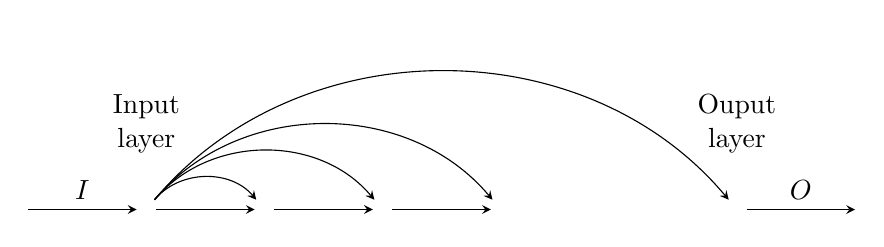
\begin{tikzpicture}[x=1.5cm, y=1.5cm, >=stealth]

\foreach \m/\l [count=\y] in {1,2,3,4,missing,5}
  \node [every neuron/.try, neuron \m/.try] (input-\m) at (1+\y ,1) {};

\foreach \l [count=\i] in {1}
  \draw [<-] (input-\i) -- ++(-1,0)
    node [above, midway] {$I$};


\draw [->] (input-5) -- ++(1,0)
    node [above, midway] {$O$};

\foreach \y [count=\yi] in {1,2,3}  
%   \foreach \j in {1,...,2}
       \pgfmathtruncatemacro{\cur}{\y}
       \pgfmathtruncatemacro{\next}{\y + 1}
      \draw [->](input-\cur) -- (input-\next);
    %   \draw [->] (input-\cur) to [out=50,in=160] (input-5);    


\foreach \y [count=\yi] in {1,2,3}  
%   \foreach \j in {1,...,2}
       \pgfmathtruncatemacro{\cur}{\y}
       \pgfmathtruncatemacro{\next}{\y + 1}
    %   \draw [->](input-\cur) -- (input-\next)
       \draw [->] (input-1) to [out=50,in=130] (input-\next);    
% \draw [->](input-1) -- (input-5);
\draw [->] (input-1) to [out=50,in=130] (input-5);

\foreach \l [count=\x from 0] in {Input, Ouput}
  \node [align=center, above] at (2 + \x*5,1.4) {\l \\ layer};
\end{tikzpicture}
\paragraph{Q2 Solution}

Proof by induction, suppose that for a chain of \( n - 1 \) neurons the \( VC \dim \) of the net \( h_{n-1} \) is \(n-1\), and denote by \(S_{n-1} \) the set which is shattered by the class, than, we could choose \( w_n \) such that \( |w_n \cdot \max_{x \in S_{n-1}}{ x } |  \le \frac{1}{2} \), of course that for every \(x \in S_{n-1} \) we get  that \[ h_n (x) = sign(w_n \cdot x + h_{n-1}(x) ) = h_{n-1}(x) \] also we could choose \( x^{\prime}\) such that \( |x^{\prime}| \ge |\frac{4}{w_n}| \) and therefore, we could determine the sign of \( w_n \) such that \( h_{n+1} ( S_{n-1} \cup \{ x^{\prime} \} ) \) will match the given classification. therefore \( S_{n} = S_{n-1} \cup \{ x^{\prime} \} \) is a set of size \( n \) which shattered by the class.

The Contradiction of the existence of shattered set at size \( n + 1 \) is given by the reverse reduction; the last neuron could not add more than \( 1 \) for the total \( VC \dim \), therefore there is must exist a shattered set at size \( n \) for the \( n - 1\) neuron chain. repeating until \( n = 1 \) leads to a contradiction.
\paragraph{Q3 Periodic function VC dim} Consider the Rectangle function over the segment \( [ 0,T] \)  as

 \[ r(x)=\begin{cases} 1 & x \in [-\frac{T}{2} ,\frac{T}{2}  ] \\ -1 & else \end{cases} \]
And define the Periodic Rectangle \( r : \mathbb{R} \rightarrow \left\{0,1\right\}  \) be an extension of the rectangle over  \( \mathbb{R} \) such that \( r (x + T) = r(x) \). 
For each of the following mark whether or not the hypothesis class \[ \mathcal{H} = \left\bigg\{ h_w\left(x\right) = r\left(w\cdot x\right) | w \in \mathbb{R} \right\bigg\} \] shatters the following samples.  
\paragraph{Q3 Solution} First note that \( h_w \) is an even function, therefore, each assignment of the form \( \{ (X_1, Y_1), (X_2,Y_2) \} \) where \( X_1 \subset \mathbb{R}^{+} \) and \(X_2 \subset \mathbb{R}^{-} \) is equivalence to assignment of the form  \( \{ (-X_1, Y_1), (X_2,Y_2) \} \).
So first, it's drop all the samples which can't be classified by an even function. 
\paragraph{Lemma} The \( VC \dim \) of Periodic function \( f \) with Periodic \( T \) over the positive axis \( \mathbb{R}^{+} \) is \( \infty 
\paragraph{Proof:} Assume that \( (X,Y) \) is a sample where \( X \) contains only rational positive numbers \( \mathbb{Q}^{+} \).Assume by induction, that there are frequencies \( w_1, w_2 \) such that \( h_{w_1} \) classify the first \( \frac{n}{2} \) points and \(h_{w_2} \) classify the other half. we will show that one can find a frequency \( w^\prime \) such that \( h_{w^\prime } \) classify \( \{X,Y\} \)  i.e:

\[ 
w^{\prime}x_{i}+m_{i}\cdot T=\begin{cases}
w_{1}x_{i} & i\le k\\
w_{2}x_{i} & else
\end{cases}
\]
Let add the following constrain \( \sum_{0}^{2k}x_{i}m_{i}=1 \) and then we will get the next matrix: 

\[
\overset{A}{\overbrace{\left[\begin{array}{ccccc}
0 & x_{1} & x_{2} & x_{3} & \cdots\\
x_{1} & T\\
x_{2} &  & T\\
x_{3} &  &  & T\\
\vdots &  &  &  & \ddots
\end{array}\right]}}\cdot\left[\begin{array}{c}
w^{\prime}\\
m_{1}\\
m_{2}\\
m_{3}\\
\vdots
\end{array}\right]=\left[\begin{array}{c}
1\\
w_{1}x_{1}\\
\vdots\\
w_{2}x_{k}\\
\vdots
\end{array}\right]
\]
We could assume without loose a generality that the points sample from the domain \( [0,T] \) ( otherwise, we could project the points in the beginning ), it follows that, A is PSD matrix: 

\begin{equation}
\begin{split} u^{T}Au	= &  \sum_{ij}a_{ij}u_{i}u_{j}= \\ & \sum{ a_{ii}u_{i}^{2}+a_{jj}u_{j}^{2}+a_{ij}u_{i}u_{j}}=  \\ &
\sum_{i,j\neq0}{T\left(u_{i}^{2}+u_{j}^{2}\right)}+\sum_{i=0}2a_{ij}{u_{i}u_{j}} \ge 0 
\end{split}
\end{equation}
Therefore, the matrix is invertible and \( m_{i}=\frac{p_{i}}{q_{i}}\in\mathbb{Q} \) ( because \( A\in\mathbb{M}\left(\mathbb{Q}\right) \) ). lets choose a numbers \( M,\alpha\in\mathbb{N} \) such that \( \alpha\left(\prod q_{i}\right)-1=M\cdot T \) and assign \( w^{\prime}\leftarrow\alpha\left(\prod q_{i}\right)w^{\prime} \) and we will get that for every \( x_j \) which classified by \( h_{w_1} \), it is also classifed by \( h_{w^\prime}} \):  
\begin{equation}
    \begin{split}
        h_{w^{\prime}}\left(x_{j}\right)  &=  sign\left(f\left(\alpha\prod q_{i}w^{\prime}x_{j}\right)\right)= \\ & sign\left(f\left(\alpha\prod q_{i}\left(w_{1}x_{j}+m_{j}T\right)\right)\right)
	=sign\left(f\left(\left(\alpha\prod q_{i}\right)w_{1}x_{j}\right)\right)= \\ & sign\left(f\left(\left(\alpha\prod q_{i}-1\right)w_{1}x_{j}+w_{1}x_{j}\right)\right)
	=sign\left(f\left(w_{1}x_{j}\right)\right)= \\ & h_{w_{1}}\left(x_{j}\right)=y_{j}
    \end{split}
\end{equation}

At the same way, it can be shown that \( h_{w^\prime}} (x_j) =  h_{w_2} (x_j)
\) for every \(x_j\) which classified by \( h_2 \). for the completeness of the proof, Its left to show that if a class of continues function shatter a set at size \(n\) over the rational numbers then it's also shatters a set at size \( n \) over the real numbers.    
\end{document}
